\section{移动机器人定位介绍}

\begin{comment}
1.机器人定位存在其位姿不能直接感知的问题,换句话说,就是大多数机器人并不拥有测量位姿的无噪声传感器。因此位姿必须从数据推断获得。
2.机器人定位不能通过自身携带的传感器直接感知。因此位姿必须从数据中推断。

\end{comment}

\begin{frame}
  \frametitle{定位问题的概念}
  \begin{columns}
    \column{0.5\textwidth}
    \begin{itemize}
      % \item 移动机器人定位就是根据给定的环境地图、环境感知和自身运动,确定自己相对于地图的位置。
      \item 移动机器人定位就是根据给定的{\color{red}环境地图}、{\color{red}环境感知}和{\color{red}自身运动},确定自己相对于地图的位置。
      \item 主要的困难:一次机器人测量不足以确定位姿。相反,机器人必须长时间整合数据以确定它的位姿。
    \end{itemize}
    \column{0.5\textwidth}
    \begin{figure}
      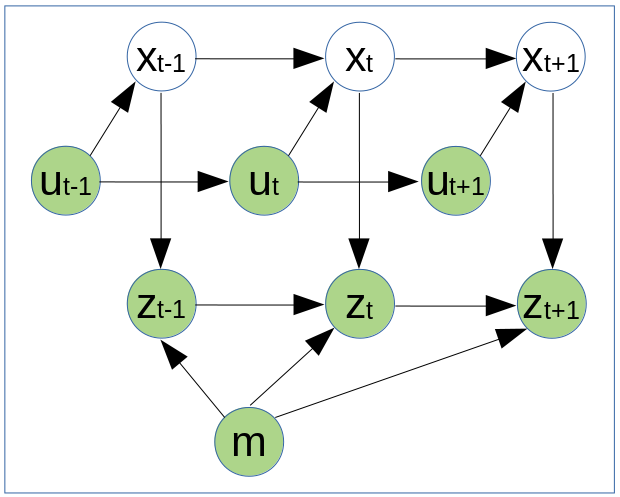
\includegraphics[height=4.0cm]{amcl/location.png}
      \caption{移动机器人定位图例模型}
    \end{figure}
  \end{columns}




  
\end{frame}



\begin{frame}
  \frametitle{定位问题的分类}
  \begin{itemize}
    \item 局部定位与全局定位
    \begin{itemize}
      \item {\color{red}局部定位};也称位姿跟踪,假定机器人初始位姿已知,通过相邻时刻传感器信息对机器人位姿进行跟踪估计。(里程计法、惯性导航法)
      \item {\color{red}全局定位};也称为重定位,机器人初始位姿未知,通过预先确定好的环境模型和传感器信息,计算机器人在全局坐标系中的位姿。(信标定位、地图匹配、GPS)
      \item {\color{red}机器人绑架};是全局定位问题的一个变种,机器人在运行过程中被绑架(瞬间被移动到其他位置)。
            绑架问题比全局定位更困难,因为机器人可能相信知道自己在哪儿,尽管它不在那里。而全局定位,机器人知道不知道自己在哪儿。
    \end{itemize}
    % \item 静态环境与动态环境
    % \item 主动定位与被动定位
    % \item 单机器人与多机器人
  \end{itemize}
  
\end{frame}

\begin{frame}
  \frametitle{定位问题的分类}
  \begin{itemize}
    \item 静态环境定位与动态环境定位
    \begin{itemize}
      \item 静态环境;定位过程中只有机器人在移动,环境里其他目标保持在同一位置。静态环境具有一些很好的数学特性,使得机器人服从高效概率估计。
      \item 动态环境;环境中除了移动的机器人外,还有动态的人、日光(对安装摄像头的机器人)、可移动的物体、门等。动态环境定位比静态环境定位更困难。
    \end{itemize}
    \item 被动定位与主动定位
    \begin{itemize}
      \item 被动定位;定位算法仅观察机器人运动。机器人通过其他方式控制,并且机器人运动不针对便于定位。比如,机器人随意移动或执行它的任务。
      \item 主动定位;定位算法控制机器人运动,以便最小化定位误差。主动定位方法往往能产生比被动定位方法更好的定位结果。
    \end{itemize}
  \end{itemize}
  
\end{frame}

\begin{frame}
  \frametitle{定位问题的分类}
  \begin{itemize}
    \item 单机器人定位与多机器人定位
    \begin{itemize}
      \item 单机器人定位;在单一机器人平台上收集所有数据,执行定位算法,不存在通信问题。
      \item 多机器人定位;机器人能相互探测,共享自身位置及传感器数据,定位有可能做的更好。
    \end{itemize}
  \end{itemize}
\end{frame}


\begin{comment}
1.表示:贝叶斯网、马尔科夫网、因子图
2.推理:精确推理和近似推理
3.参数学习

1.最速下降:负梯度方向搜索,收敛速度慢。
2.Newton法:保留了泰勒展开的一阶和二阶项,二次收敛速度,但每步都需要计算法Hessian矩阵,复杂的高。
3.GN法:通过Jacobian矩阵近似H矩阵,提高了算法的效率,但H矩阵不满秩则无法迭代。
4.LM法:基于信赖域算法,解决H矩阵不满秩或非正定问题。

\end{comment}
\begin{frame}
  \frametitle{定位问题的求解}
  \centering
  \fbox{
  \parbox{0.8\textwidth}{
    \begin{center}
      定位问题求解大致分为两类:滤波方法和优化(图优化)方法。
    \end{center}
    }
  }
  \begin{columns}
    \column{0.5\textwidth}
    \begin{figure}
      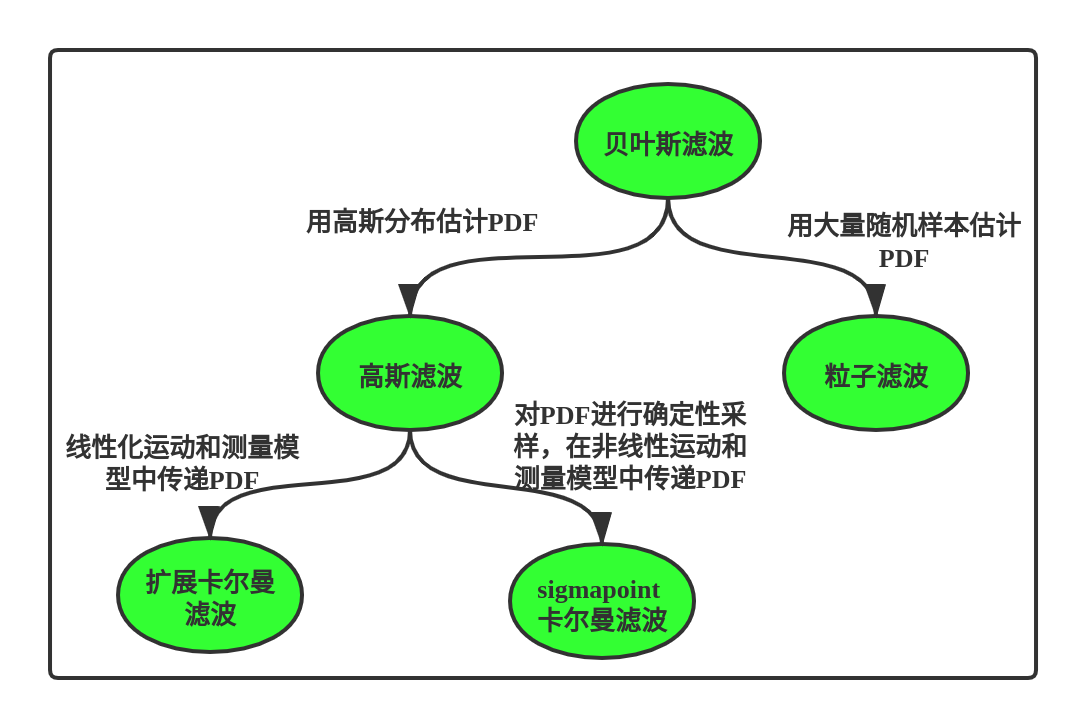
\includegraphics[height=4.0cm]{amcl/filter.png}
      \caption{滤波方法定位}
    \end{figure}
    \column{0.5\textwidth}
    \begin{figure}
      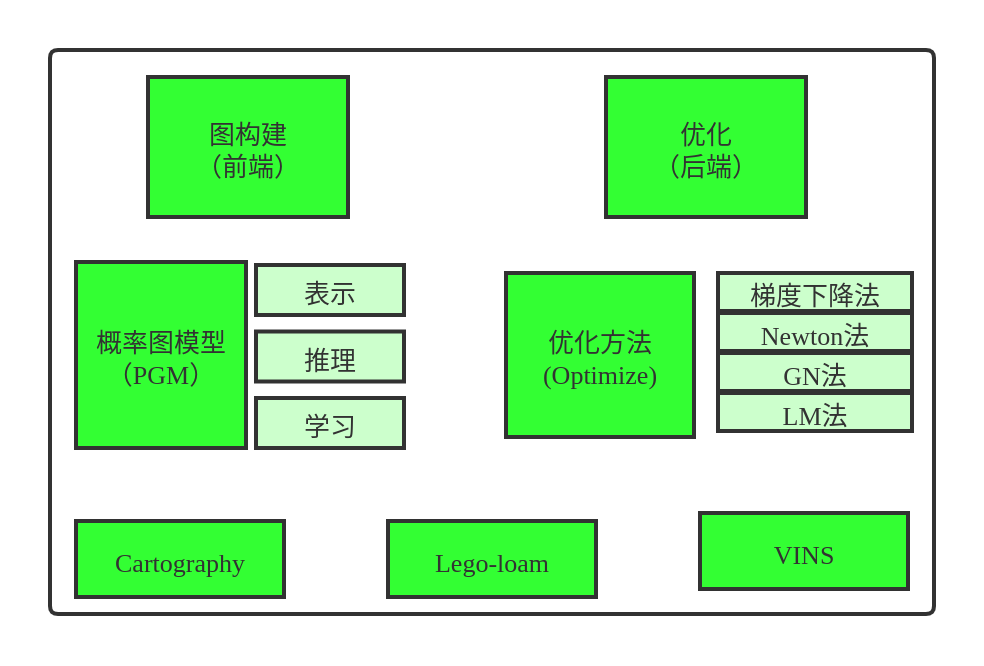
\includegraphics[height=4.0cm]{amcl/optimize.png}
      \caption{图优化方法定位}
    \end{figure}
  \end{columns}


\end{frame}




\begin{comment}
蒙特卡罗方法也称统计模拟方法,通过采样来获得目标分布。从而将数值计算问题转化为概率统计的方法。
MCMC是很多算法求解的基础,在机器学习和强化学习都有广泛的应用

MC:解决难以用数值计算的问题转换为概率统计的方法

感知、定位、建图包含很深的理论。

MCMC采样
\end{comment}

\begin{frame}
  \frametitle{自适应蒙特卡罗定位(AMCL)}
  \begin{columns}
    \column{0.5\textwidth}
    \begin{itemize}
      \item 蒙特卡罗方法(MC):也称统计模拟方法,通过采样来获得目标分布,采样方式包括了{\color{red}概率分布采样}、接受-拒接采样和Gibbs采样等。
      \item 蒙特卡洛定位(MCL):是一种用粒子表示机器人位姿置信度$bel(x_t)$的定位算法。
    \end{itemize}
    \column{0.5\textwidth}
    \begin{figure}
      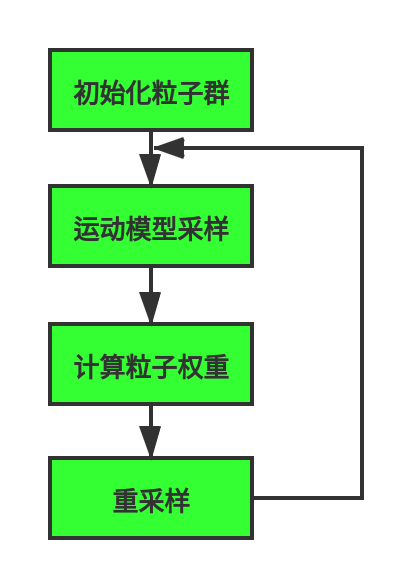
\includegraphics[width=3.5cm]{amcl/mcl.png}
      \caption{MCL算法流程}
    \end{figure}
  \end{columns}

\end{frame}

\begin{comment}
1.这里介绍一种能够实现自动调节粒子数量的算法-库尔贝克-莱布勒散度。

2.熵:

如果对深度学习有了解的话,深度学习的损失函数中有一个交叉熵的概念。
!!交叉熵是深度学习中常用的一个概念。用在损失函数中求目标与预测值之间的差距。
信息论:熵--信息量,
信息量应该和事件发生的概率有关; $I(x_0) = -\log(p(x_0))$
当越不可能的事件发生了,我们获取到的信息量就越大;
!!熵用来表示所有信息量的期望; $H(X) = - \sum_{i=1}^n p(x_i)\log(p(x_i))$

3 相对熵(KL散度)
对于同一个随机变量 x 有两个单独的概率分布 P(x) 和 Q(x),
我们可以使用 KL 散度(Kullback-Leibler (KL) divergence)来衡量这两个分布的差异

\end{comment}

\begin{frame}
  \frametitle{自适应蒙特卡罗定位(AMCL)}
  \begin{itemize}
    \item 对于粒子滤波器的效率来说,用于表示置信度采样集的大小是一个重要的参数。在定位的早期阶段高的粒子数可能是定位所必须的,
          但是一旦知道机器人在哪里,仅需要一小部分粒子就足以跟踪机器人的位姿。
    \item {\color{red}库尔贝克-莱布勒散度}(Kullback-Leiber Divergence,KLD),也称为相对熵(relative entropy),是描述两个概率分布P和Q差异的一种方法。
          在信息论中,$D(P||Q)$表示当用概率分布Q来拟合真实分布P时,产生的信息损耗。
    \item 对于一个离散随机变量的两个概率分布P和Q来说,他们的KL散度定义为:
          $$D(P||Q) = 
          \sum_{i=1}^N p(x_i) \cdot \log \frac{p(x_i)}{q(x_i)} = 
          \sum_{i=1}^N p(x_i) \log(p(x_i)) - \sum_{i=1}^N p(x_i)\log(q(x_i))$$
  \end{itemize}
  
\end{frame}

\begin{frame}
  \frametitle{AMCL算法}

  \begin{columns}
    \column{0.1\textwidth}
    \column{0.8\textwidth}
    \begin{block}
      
    \begin{algorithmic}[1]

      \State Algorithm AMCL$(\mathcal{X}_{t-1}, u_t, z_t, m, \epsilon, \sigma)$
      \State $\mathcal{X}_t = \emptyset, M = 0, M_{\mathcal{X}} = 0, k = 0$
      \State for all b in H do  
      \State \quad $b = empty$
      % \State endfor
      \State do
      \State \quad draw i with probability $\propto w_{t-1}^{[i]}$
      \State \quad $x_t^{[M]} = \text{sample\_motion\_model}(u_t, x_{x-1}^{[i]})$
      \State \quad $w_t^{[M]} = \text{measurement\_model}(z_t, x_t^{[M]}, m)$
      \State \quad $\mathcal{X}_t = \mathcal{X}_t + \left\langle x_t^{[M]}, w_t^{[M]} \right \rangle$
    \end{algorithmic}
    \end{block}

    \column{0.1\textwidth}
  \end{columns}
\end{frame}

\begin{frame}
  \frametitle{AMCL算法}

  \begin{columns}
    \column{0.1\textwidth}
    \column{0.8\textwidth}
    \begin{block}
      
    \begin{algorithmic}[1]

      \State \quad $\text{if } x_t^{[M]} \text{ falls in empty bin b then}$  \textit{
        \tiny // 如果新产生的粒子落入直方图的一个空位里} %\textbf{//}
      \State \qquad $k = k+1$ 
      \State \qquad $b = \text{non-empty}$
      \State \qquad $\text{if } k > 1 \text{ then}$ \textit{\tiny  // 粒子越分散,越多的空位被填满,计算得到$M_{\mathcal{X}}$就越大}
      \State \qquad \quad $M_{\mathcal{X}} := \frac{k-1}{2\epsilon} \left\{1 - \frac{2}{9(k-1)} + \sqrt{\frac{2}{9(k-1)}}z_{1-\sigma} \right\} ^3$
      \State \qquad $M = M + 1$
      \State $\text{while } M < M_{\mathcal{X}} \ or \ M < M_{\mathcal{X}min}$
      \State return $X_t$
    \end{algorithmic}
    \end{block}

    \column{0.1\textwidth}
  \end{columns}
\end{frame}

% \text{}
% {\color{Blue} aa}
% \begin{frame}
%   \frametitle{AMCL算法}

%   \begin{columns}
%     \column{0.1\textwidth}
%     \column{0.8\textwidth}
%     \begin{block} 
%     \begin{algorithmic}[1]

%       % \State \quad $\text{if } x_t^{[M]} \text{ falls in empty bin b then} $ \sum
%       % \State \quad $x_t^{[M]} = \text{sample\_motion\_model}(u_t, x_{x-1}^{[i]})$
%       % \State \quad $w_t^{[M]} = \text{measurement\_model}(z_t, x_t^{[M]}, m)$
%       % \State \quad $\mathcal{X}_t = \mathcal{X}_t + \left\langle x_t^{[M]}, w_t^{[M]} \right \rangle$
%     \end{algorithmic}
%     \end{block}

%     \column{0.1\textwidth}
%   \end{columns}
% \end{frame}

% \begin{frame}
%   \frametitle{定位问题概念}
%   \begin{itemize}
%     \item 
%   \end{itemize}
  
% \end{frame}

